
\chapter{Результаты}\label{chapt4}

\section{Спектрометр протонов и электронов}
Прибор СПЭ содержит четыре одинаковых четырех-детекторных телескопа, устройства аналоговой и цифровой обработки сигналов детекторов, интерфейсные устройства, источники вторичного напряжения. 

Структурно аппаратура разделяется на Детекторные Блоки и Блок Обработки Данных. Блок обработки данных выступает как интерфейсный блок с бортовой аппаратурой КА и телеметрией, а детекторные блоки  в свою очередь, связаны кабельной сетью с блоком обработки данных.

Основным элементом детекторного блока являются детекторные сборки - телескопы, состоящие из полупроводниковых детекторов различной толщины и сцинтилляционного детектора, расположенных один под другим, которые регистрируют попадающие в них частицы. Оси телескопов из различных детекторных блоков расположены под углом $ 109^\circ28'  $друг относительно друга. 

Рисунок 4.2. Структурная схема детекторного блока прибора СПЭ. Сверху указано количество устройств данного типа в детекторном блоке.
.

На  рис. 4.2 представлена структурная схема одного детекторного блока. Детекторы каждого телескопа производят электрические импульсы, амплитуда которых пропорциональна энерговыделению в детекторах, далее эти импульсы через эмиттерный повторитель поступают на вход зарядочувствительного усилителя, который усиливает сигналы до величин, позволяющих производить с помощью компараторов выделение энергетических порогов.

В детекторных блоках находятся электронные логические устройства отбора, работающие на принципе совпадений и антисовпадений электрических импульсов. Данные логические устройства отбора реализуют условия, позволяющие раздельно регистрировать электроны и протоны ОКП и получать энергетические распределения (зависимость потоков частиц от энергии) этих частиц в пространстве и во времени.  Дополнительно в функции этого логического устройства, входит счетчик, обеспечивающий регистрацию количества событий, удовлетворяющих условиям отбора конкретного логического устройства. Данные со счетчиков за определенный момент времени записываются в оперативное запоминающее устройство (ОЗУ), обеспечивающее запоминание первичных данных по зарегистрированным частицам. 

Данные из ОЗУ детекторного блока поступают в постоянное запоминающее устройство (ПЗУ) блока обработки данных, в котором собирается и хранится информация со всех детекторных блоков и, после специальной сортировки, по мультиплексному каналу информационного обмена (МКИО) поступает в бортовые системы МКА. В следующем параграфе приведены структурные схемы логических схем отбора событий, реализованные по результатам моделирования. 

\subsection{Разработка структурных схем блоков аппаратуры радиационного контроля ОКП и описание принципов их работы}

Разработка структурных схем блоков аппаратуры радиационного контроля ОКП проводилась путем моделирования работы цифровых и аналоговых узлов прибора СПЭ (телескопическая система) в среде Simulink (MATLAB), с использованием данных численного моделирования детектирующей части прибора в среде Geant4. 
Simulink – это графическая среда имитационного моделирования, позволяющая при помощи блок-диаграмм в виде направленных графов строить динамические модели, включая дискретные, непрерывные и гибридные, нелинейные и разрывные системы. Дополнительные пакеты расширения Simulink позволяют решать спектр задач от разработки концепции модели устройства до тестирования, проверки, генерации кода и аппаратной реализации [1].

Simulink интегрирован в среду MATLAB, что позволят использовать встроенные математические алгоритмы, такие как расчет параметров распределения Пуассона, что будет продемонстрировано в разделе 3.2

\subsection{ Описание электронной модели прибора СПЭ}

Электронная модель прибора СПЭ создавалась с использованием как стандартных блоков Simulink, так и специализированных блоков для программирования промышленно выпускаемых программируемых логических интегральных схем (ПЛИС), представлена на рисунке \ref{fig:simulink}.

\begin{figure}
\centering
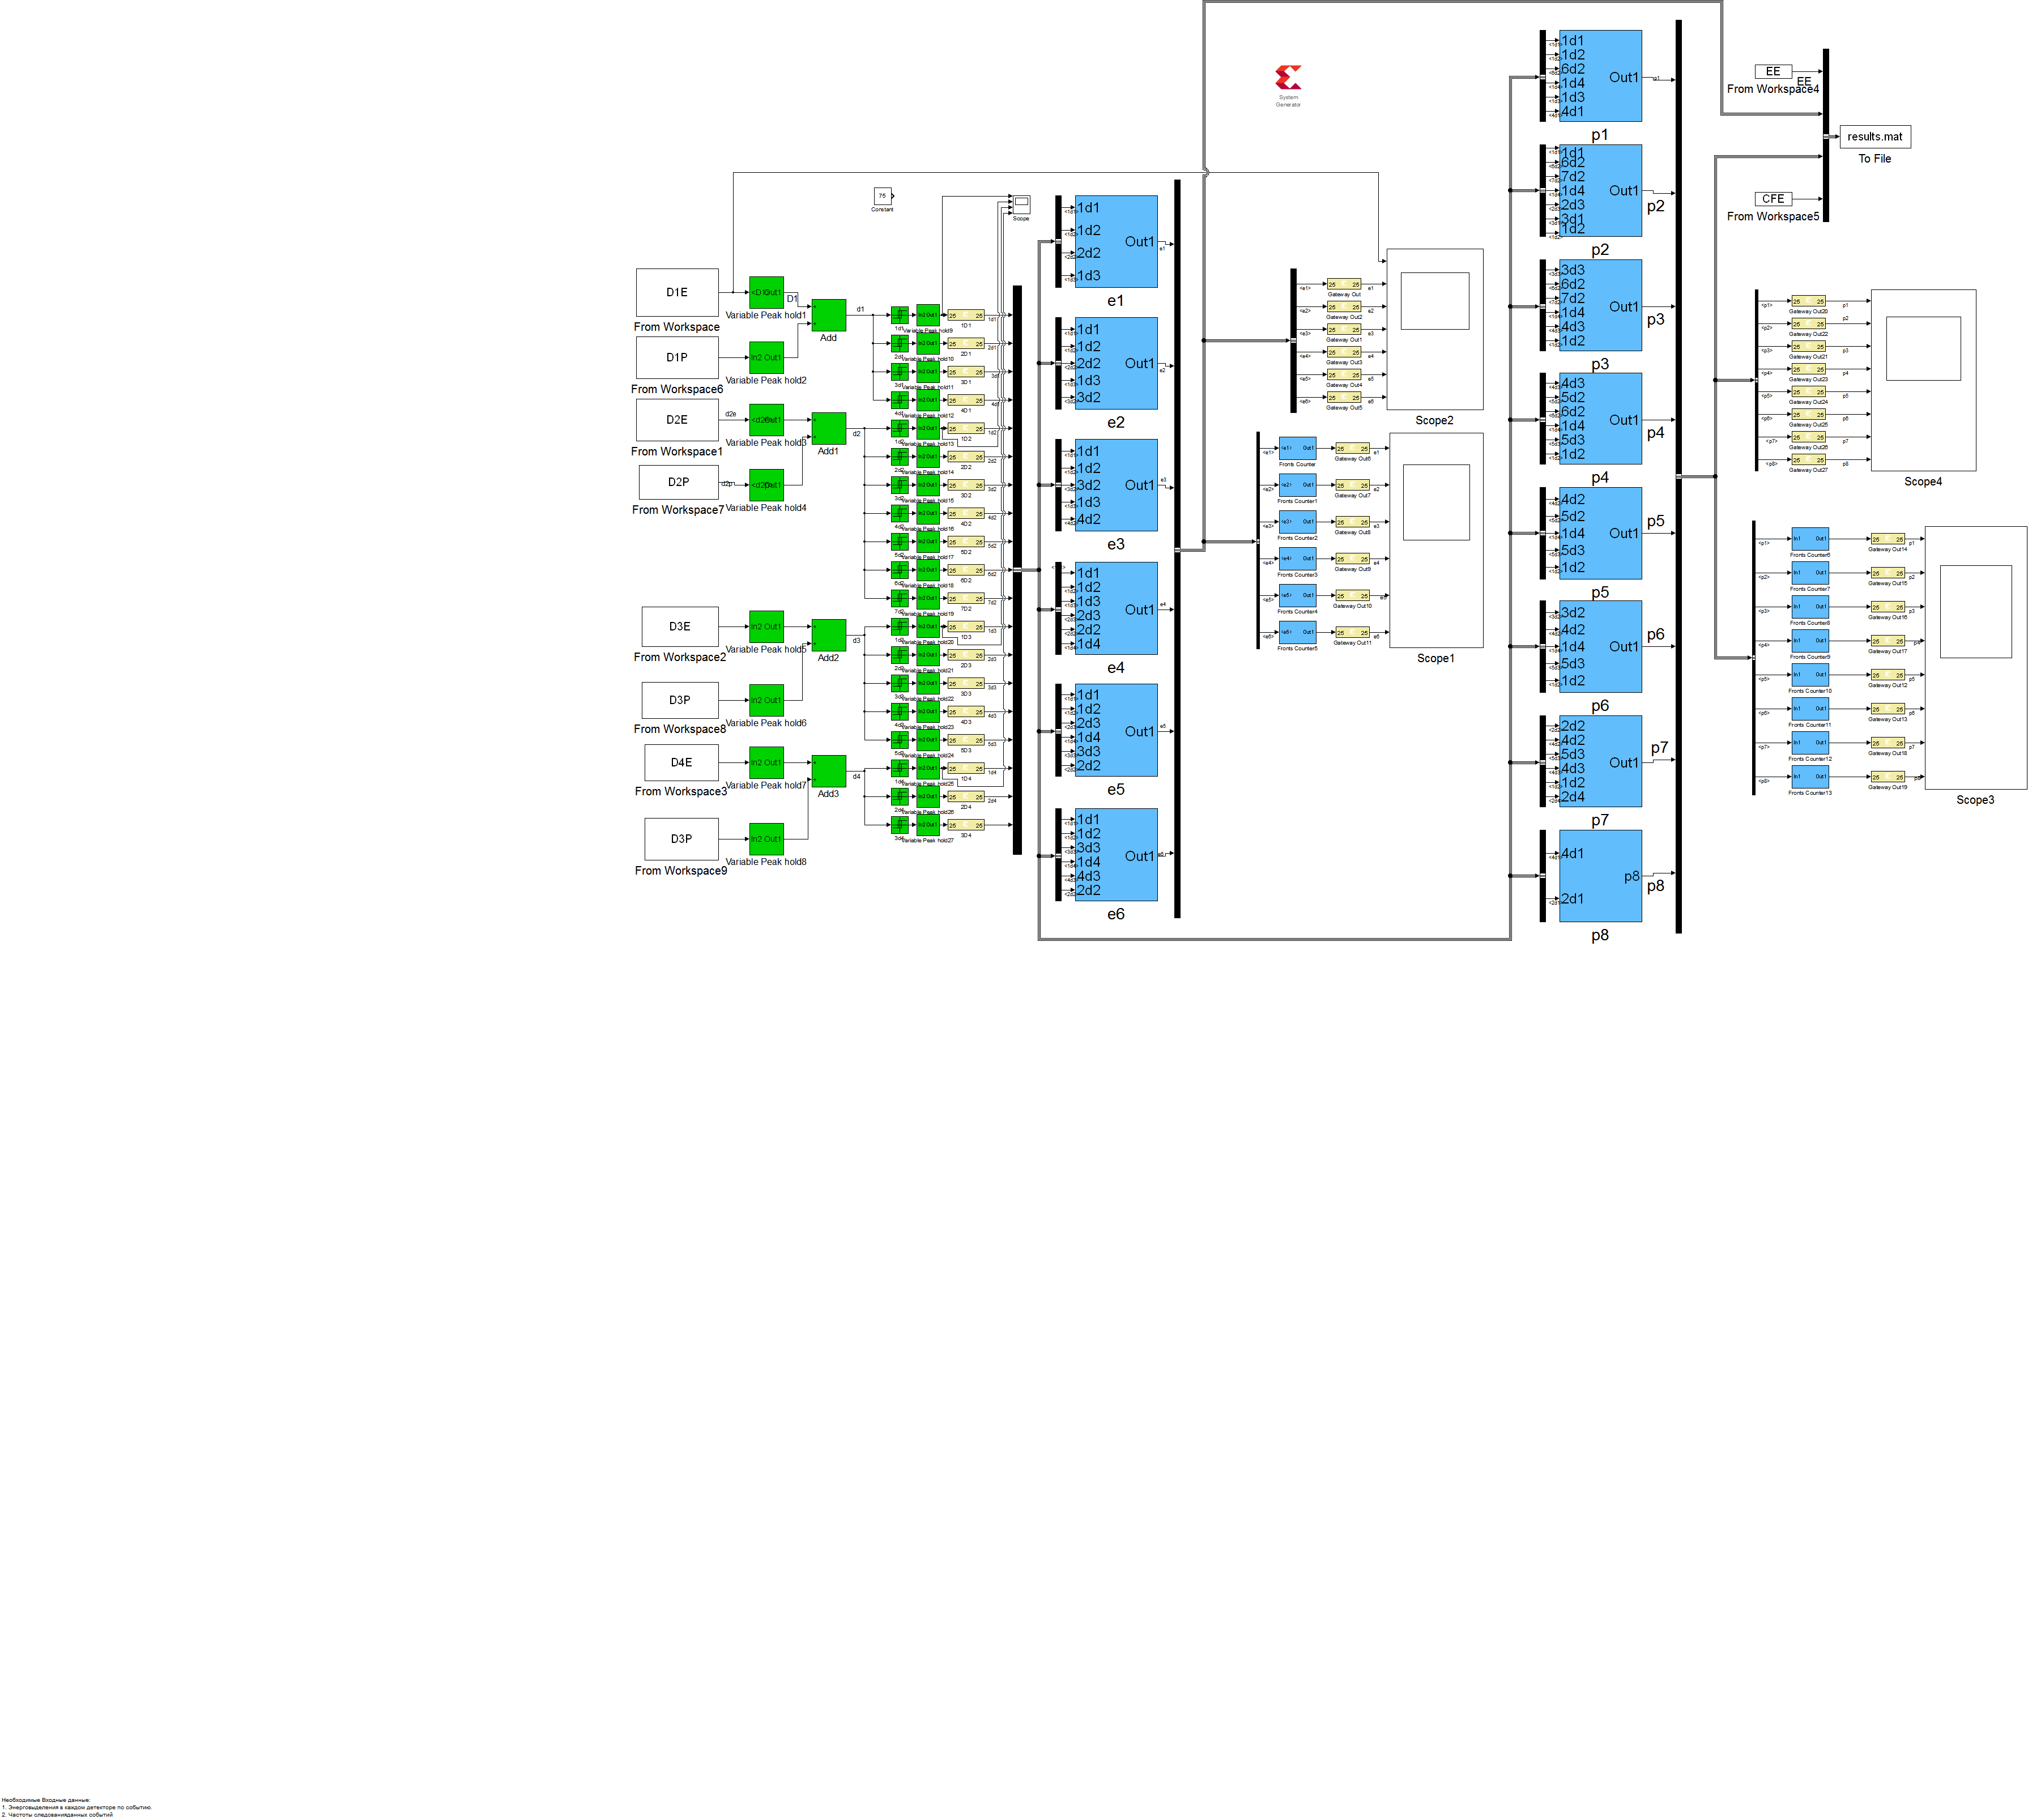
\includegraphics[width=0.7\linewidth]{images/simulink}
\caption{Общий вид модели прибора СПЭ в среде Simulink/Matlab. Логика определения типа и энергии частиц сгруппирована в подсистемы: е1-е6 структурные схемы выделения элекронов,  p1-p8 структурные схемы выделения протонов. D1…4E – промоделированные массивы энерговыделений в детекторах от электронов, D1…4P -  промоделированные массивы энерговыделений в детекторах от протонов. Блоки scope1-scope4 – виртуальные осциллографы в среде MATLAB, обеспечивающие наглядное отображение реакции исследуемого устройства на задаваемые внешние сигналы. Зеленым цветом показаны подсистемы имитации аналоговых сигналов, голубым цветом – подсистемы предназначенные для трансляции в аппаратный код ПЛИС, желтым цветом – выводы ПЛИС.}
\label{fig:simulink}
\end{figure}

При построении электронной модели прибора из стандартной библиотеки блоков Simulink были использованы:
1.	 блок “From Workspace”, позволяющий импортировать подготовленные массивы входных данных об энерговыделениях в детекторах;
2.	блок “To File”, позволяющий экспортировать в структурированный файл (формата .MAT) массивы выходных данных логических счетчиков;
3.	блок “Scope”, позволяющий проводить визуализацию массивов и строить графики промежуточных результатов вычислений в режиме реального времени;
4.	блок определения изменения уровня сигнала “Detect Change”, формирования преключателей “Switch” и имитации реальных длительностей сигналов от формирователей аналоговой части прибора путем реализации задержки сигнала “Zero-order Hold”. Эти блоки  экспортируются только в подсистемы имитации аналоговых сигналов (рис. 3.2);
5.	блок «Relay», имитирующий работу компараторов аналоговой части прибора и настраиваемый на пороговые значения включения и выключения, соответствующие энергетическим порогам прибора СПЭ.
А также другие блоки из стандартной библиотеки Simulink.

\begin{figure}
\centering
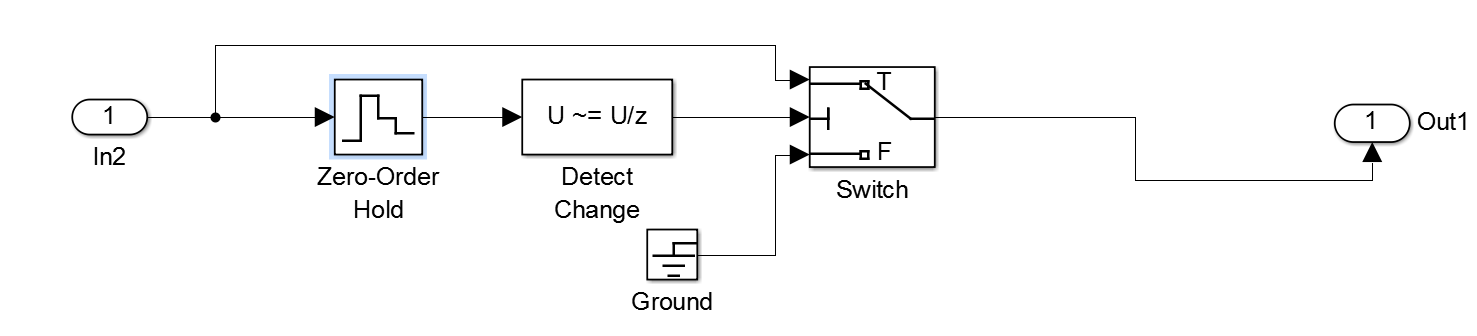
\includegraphics[width=0.7\linewidth]{images/simulink_analog}
\caption{Подсистема имитации аналоговых сигналов, формирования импульсов сигналов длительностью в 1 такт.}
\label{fig:simulink_analog}
\end{figure}


На входы модели при моделировании подавались величины энерговыделений в детекторах, полученные в результате Монте-Карло моделирования прибора СПЭ (раздел 2). Так как при моделировании в Geant4 каждое событие считается независимым от остальных, для использования этих данных в среде Simulink требуется вводить дополнительную временную характеристику, определяющую частоту срабатываний компараторов аналоговой части прибора, что будет подробно рассмотрено в разделе 3.3. 
Входные данные были разделены в файлы по типу частиц и, так как в реальных условиях работы прибор будет находиться в условиях облучения протонами и электронами КИ одновременно, в модели производится смешивание потоков этих данных путем суммирования (рис.\ref{fig:simulink_summ}).
\begin{figure}
\centering
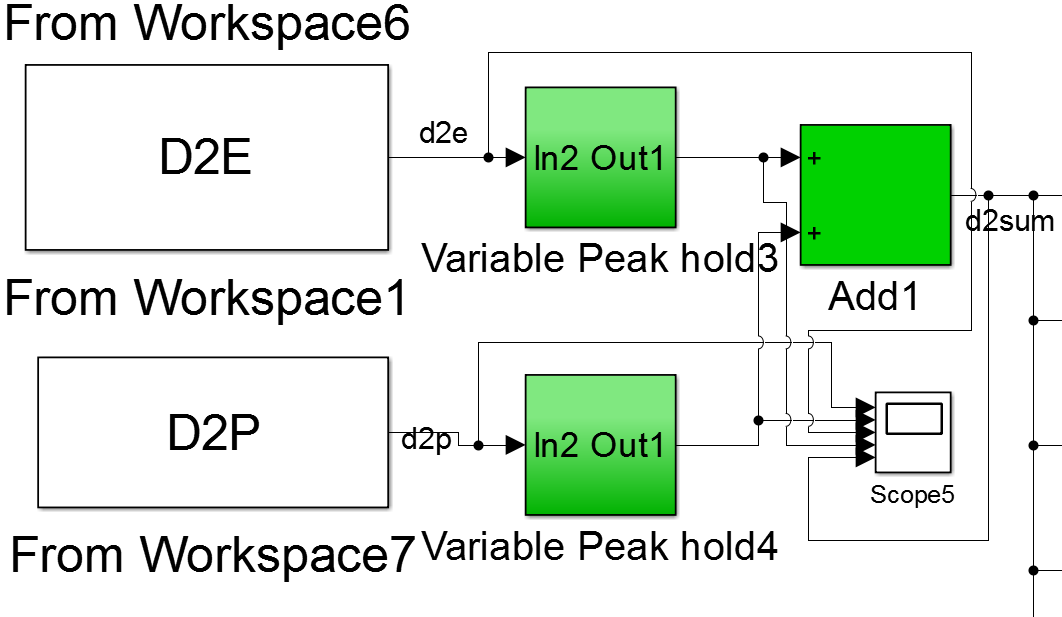
\includegraphics[width=0.7\linewidth]{images/simulink_summ}
\caption{Смешивание сигнала в детекторе 2 прибора СПЭ. «Variable Peak hold» - Подсистема формирования импульсов сигналов длительностью в 1 такт, «Scope5» – виртуальный осциллограф, «From Workspace» - ввод данных по энерговыделениям в детекторах, «Add1» - сумматор}
\label{fig:simulink_summ}
\end{figure}






Подсистема формирования импульсов сигналов длительностью в 1 такт требуется для верного последующего смешивания сигналов. Ввод данных по энерговыделениям в детекторах происходит таким образом, что образуется ступенчатая функция, представленная на рисунке 3.4 в изображениях d2p и d2e, с длительностью ступени, зависящей от параметров распределения Пуассона. Из рисунка 3.4 видно, что временные параметры для электронов гораздо меньше по длительности, чем для протонов. Суммирование сигналов такой формы привело бы к просчету части событий регистрации электронов, поэтому смешивание происходит на фронтах входных сигналов от электронов и от протонов.
Пример работы системы имитации аналоговой части прибора изображен на рис. 3.4 (графики получены с помошью осцилогорафа рис 3.3), суммированный сигнал показан последним. Видны многократные прохождения через детектор электронов и одно прохождение протона. 

Рисунок 3.4 Моделирование работы аналоговой части детектора 2 прибора СПЭ, d2e – энерговыделение от электронов КИ, d2p - энерговыделение от протонов КИ, d2e+фильтр и d2р+фильтр – входные данные по энерговыделениям после выделения фронтов,  d2sum – итоговое энерговыделение в детекторах прибора. Временной параметр выражен в единицах тактовых сигналов ПЛИС (длительность 40нс)
После формирования смешаный сигнал поступает на группу блоков 1d2…. nd2 (рис. 3.5), имитирующих работу компараторов. Для каждого блока типа  nd2 подбирались индивидуальные значения порогов срабатывания, в соответствии с итогами определения этих параметров в разделе 3.3. Блоки nd2 производят на выходах двоичные сигналы (0 при значении на входе блока менее порога и 1 при превышении порога), пригодные для дальнейшего цифрового преобразования. Кроме того, полученные на выходах компараторов сигналы требуют формирования сигналов длительности 3 мкс для полного соответствия с принципом работы аналоговой части прибора, определяемой характерными значениями RC цепей детекторов. Цепочка преобразования сигналов показана на рисунке 3.5.

\begin{figure}
\centering
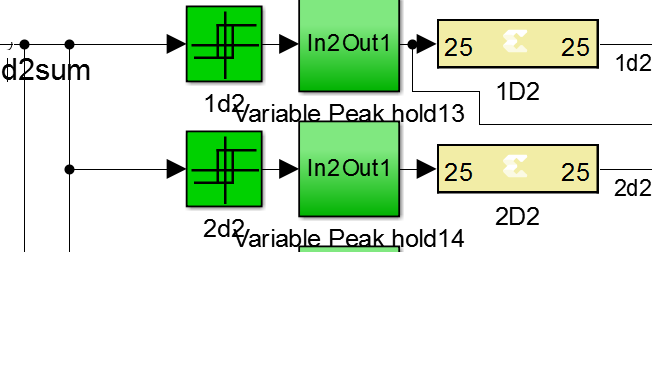
\includegraphics[width=0.7\linewidth]{images/sim_comparators}
\caption{Подсистемы имитации компараторов (1d2 и 2d2) и формирователей длительности цифровых сигналов(Variable Peak Hold13-14 )
	Подсистема имитации реальных длительностей цифровых сигналов от формирователей аналоговой части прибора выделена от остальной модели и предназначена для формирования цифровых сигналов с длительностью 3мкс, (рис. 3.6), выраженное в числе тактовых сигналов равно 75. Для канала 1Д2 (стробирующий канал, наличие которого является сигналом для всех каналов к запуску обработки) использована длительность в 400 нс для обеспечения необходимого времени работы схем отбора событий.}
\label{fig:sim_comparators}
\end{figure}


\begin{figure}
	\centering
	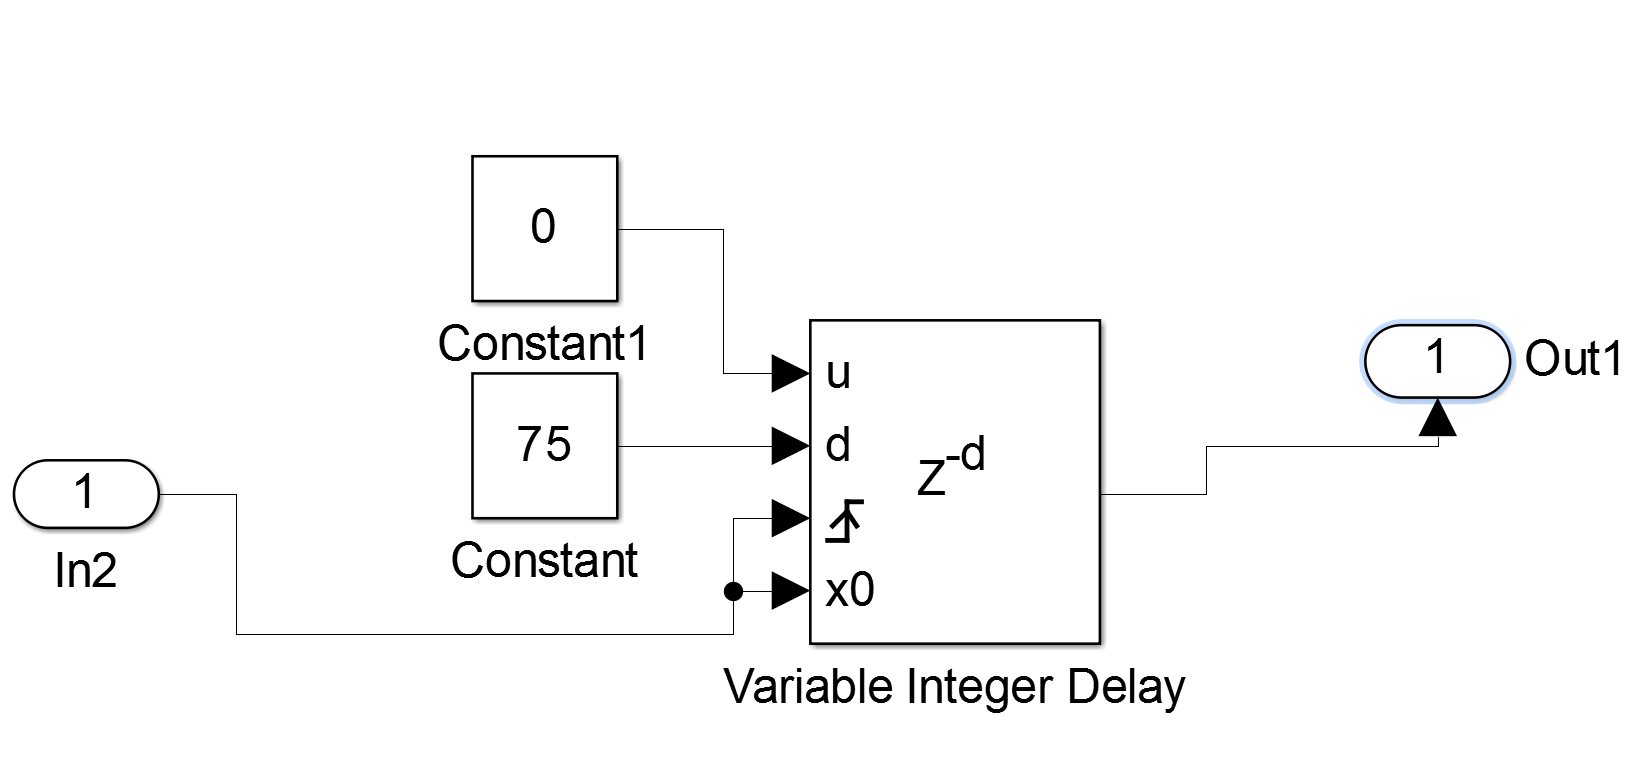
\includegraphics[width=0.7\linewidth]{images/sim_form1}
	\caption{}
	\label{fig:sim_form1}
\end{figure}
\begin{figure}
	\centering
	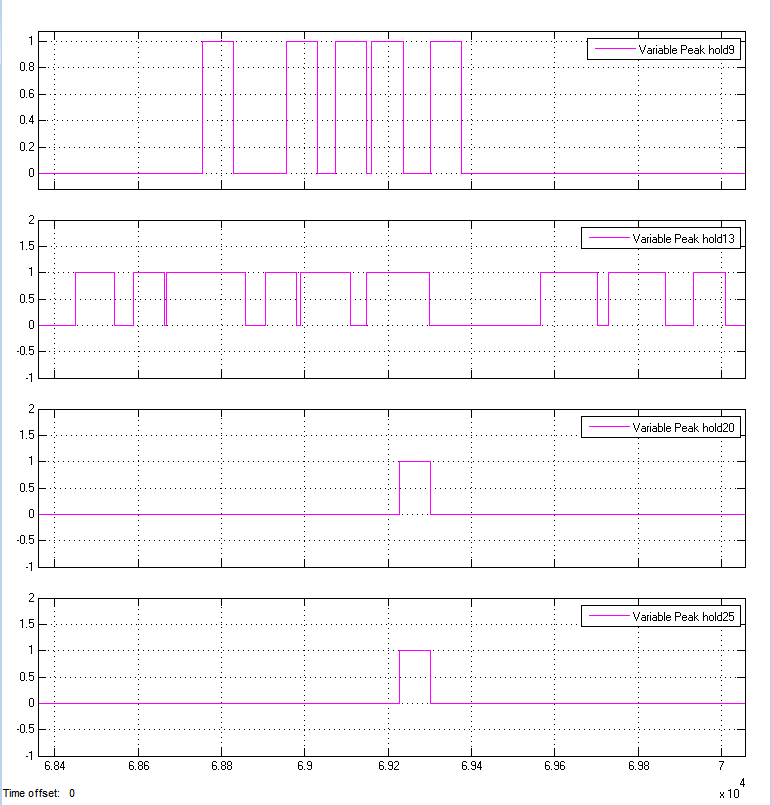
\includegraphics[width=0.7\linewidth]{images/sim_form2}
	\caption{Подсистема имитации формирователей аналоговой части прибора, использующая блоки постоянных значнией “Constant”, и задержки сигнала “Variable Integer Delay”. Ниже показан сформированный импульс длительностью 3 мкс (75 тактов несущей частоты ПЛИС)}
	\label{fig:sim_form2}
\end{figure}

После аналоговых преобразований сигналы поступают на цифровую обработку для отбора событий по определенным признакам, которая реализуется в ПЛИС. Логика цифровых преобразований в ПЛИС  реализуется с помощью элементов библиотеки Xilinx Blockset. В данной библиотеке cоздана модель отбора событий, подходящая для определения типа частицы и измерения энергетических параметров данной частицы. В состав элементов библиотеки Xilinx Blockset входит набор наиболее часто встречающихся при разработке ПЛИС элементов логики (И, ИЛИ, НЕ и тд.), элементов с двумя устойчивыми состояниями, мультиплексоры, шифраторы и дешифраторы, наборы различного типа регистров. Блоки каждого канала отбора событий по энерговыделениям были сгруппированы в подсистемы:
e1-e6 каналы выделения параметров электронов, 
р1-р8 каналы выделения параметров протонов. 
Подробный состав каждой подсистемы в виде структурных схем блоков аппаратуры радиационного контроля приведен в разделе 4.
Разработка микропрограммы для прошивки ПЛИС с использованием средств Simulink и Xilinx Blockset происходит в несколько этапов:
1.	Производится составление структурных схем модели.
2.	Производится тестирование работоспособности модели в среде Simulink.
3.	Корректируются структурные схемы с учетом результатов моделирования.
4.	Код модели экспортируется в аппаратно независимый код в формате VHDL.
5.	Полученный код VHDL используется для прошивки ПЛИС.
6.	Производится одновременная симуляция работы программы в среде Simulink и в ПЛИС.
7.	Производится корректировка кода VHDL по результатам симуляции.

Блоки библиотеки Xilinx Blockset оптимизированы для работы с устройствами производства Xilinx, аппаратный код VHDL пригоден для использования и на ПЛИС других производителей, с условием обеспечения архитектурной совместимости целевых ПЛИС с ПЛИС производства Xilinx. Такой метод позволяет после переноса кода рассчитывать на возможность использования полученных микропрограмм для ПЛИС российского производства.


\section{Подбор параметров отбора событий}

Одной из целей данного моделирования является выяснение границ энергетических каналов (электронных и протонных), подходящих для измерения прибором СПЭ. В соответствии с ТЗ энергетический диапазон измеряемых электронов должен составлять 0,15-10,0 МэВ и должен измеряться в 4-6 энергетических интервалах. В качестве первого приближения, рассмотрены интервалы с приблизительно логарифмическим шагом по энергии (таблица \ref{tab:elec_channel}).

\begin{table}
	\begin{tabular}{p{4.7cm}|cccccc}
№ канала&	Е1&	Е2&	Е3&	Е4&	Е5&	Е6\\ \hline
Границы интервалов, МэВ&	0,15-0,35&	0,35 - 0,6&	0,6-1,0&	1,0-2,0&	2,0-4,0&	4,0-10,0 
\end{tabular}
	\caption{Предварительные энергетические интервалы измеряемых энергий электронов для телескопа СПЭ.}
	\label{tab:elec_channel}
\end{table} 


На подготовительном этапе работ для электронов и протонов были выбраны предварительные границы порогов энерговыделений для каждого детектора и выбрано количество необходимых интервалов регистрации по первичным энергиям исходя из требований ТЗ. 
\subsection{Классический метод определения порогов по энерговыделению}
В таблице 3.2 приведены предварительные энергетические пороги компараторов детекторов телескопа СПЭ, подобранные классическим методом при рассмотрении зависимостей энерговыделений в детекторах определенной толщины от энергий первичных электронов. Основной предпосылкой данного метода является осевое приближение - рассмотрение только тех заряженных частиц, траектории которых минимально отклоняются от нормальных по отношению к плоскости всех детекторов. 
\todo{ссылка на книгу гольштейн?} 

Таблица 3.2 - Предварительные пороги энерговыделений в энергетических единицах для компараторов детекторов телескопа СПЭ

\subsection{Статистический метод определения порогов по энерговыделению}
Так как распространение заряженных частиц в теле детектора имеет стохастический характер и даже для моноэнергетической линии имеет вид кривой Ландау, с наложенной на нее гауссовой функцией (\ref{eq:landau}), очевидно что классический подход к подбору порогов дает весьма посредственную точность.Типиный вид данной кривой представлен на рисунке \ref{fig:landau}
\todo{Акимов Ю.К. и др. Полупроводниковые детекторы в экспериментальной физике}

\begin{equation} \label{eq:landau}
f(\Delta E, x) = \frac{1}{2\pi\sqrt{\sigma}} \int\limits_{-\infty}^{\infty}{f(\Delta E', x))e^{\frac{-\Delta E - \Delta E'}{2\sigma^2}}d(\Delta E')}
\end{equation}

где $ \delta E $ энергетические потери в веществе толщиной $ x $


\begin{figure}
\centering
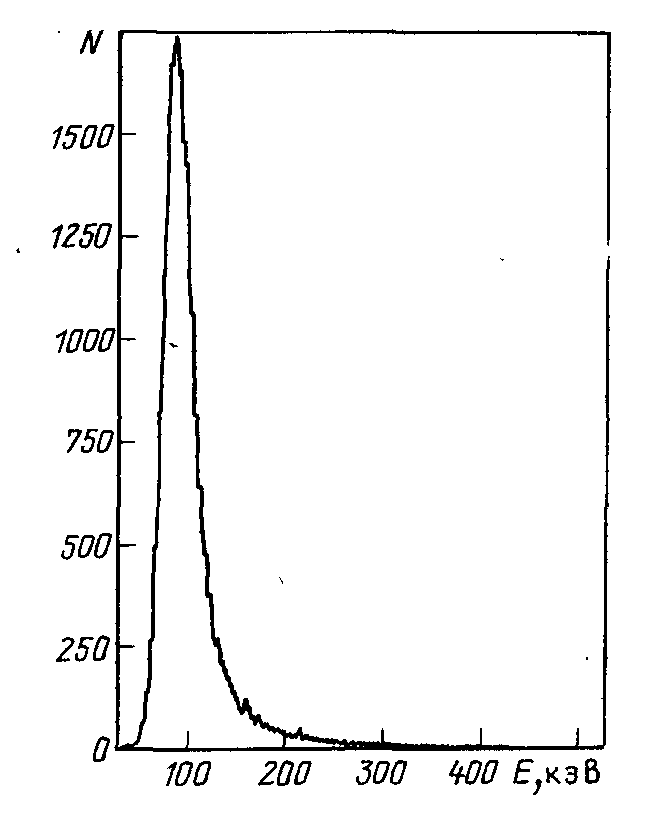
\includegraphics[width=0.7\linewidth]{images/landau}
\caption{}
\label{fig:landau}
\end{figure}






\section{Подбор временных параметров моделирования}

Как было изложено выше, при моделировании в Geant4 каждое событие считается независимым от остальных событий. Для использования данных моделирования требуется вводить дополнительную временную характеристику, определяющую частоту срабатываний компараторов аналоговой части прибора. Тем не менее, возможно получить информацию о средней частоте регистрации частиц в приборе, основываясь на итогах моделирования в Geant4, путем учета всех типов событий (в пределах коллиматора и боковые события), имеющих ненулевое энерговыделение в детекторах при этом моделировании. Эти модельные данные необходимо соотнести с реальными интегральными потоками на выбранных орбитах, получая среднюю частоту регистрации событий максимально приближенной к реальным условиям работы прибора.
Известно, что временное распределение регистрации частиц КИ соответствует распределению Пуассона, с параметром, равным среднему временному интервалу между моментами регистрации частиц [3].
В таблице 3.11 приведены рассчитанные по формуле 1 параметры распределения Пуассона, задающие временное распределение срабатываний детекторов прибора от электронов (потоки протонов значительно меньше). При расчете использовался геометрический фактор – отношение зарегистрированных частиц к общему потоку при моделировании (n/N), а также расчетные интегральные потоки на целевых орбитах и площадь модельного источника частиц, связывающая данные величины:
(1)
где t – средний период регистрации частиц при моделировании
N - общее количество частиц при моделировании;
n - количество зарегистрированных детекторами частиц при моделировании;
F(>E) – интегральный поток частиц КИ (электронов) на выбранных орбитах;
S – площадь источника частиц (прибор помещен в центр сферы с изотропным потоком излучения). 

При расчетах использовались следующие значения параметров:
•	N = 2,00E+08 частиц было запущено с поверхности сферы,
•	S = 6,08E+01 см2 – площадь источника частиц при моделировании,
•	F(>E) – интегральный поток частиц КИ (электронов) на выбранных орбитах.

В таблицах 3.11 -3.113 введены обозначения:
•	nA, nB, nC – количество частиц, выделивших энергию в детекторах прибора для различных типов корпуса прибора,
•	tA, 	tB, 	tC - рассчитанные временные параметры распределения Пуассона для различных типов корпуса прибора
Варианты материала корпуса (1 на Рис. 2.1):
•	вариант А - латунь;
•	вариант В – дюралюминий;
•	вариант С - выше пунктирной линии – латунь, ниже – дюралюминий.
Таблица 3.11 -Параметры распределения Пуассона для модельных потоков электронов
\begin{table}
	\begin{tabular}{cccccccc}
	Обозначение орбиты & F(E>	0,15 МэВ)	& nA & nB & nC & tA, с & tB, с & tC, с \\ 
	1700 км & 6,40E+07 & 1,13Е+05 & 1,09Е+05 & 1,17Е+05 & 4,52E-07 & 4,68E-07 & 4,37E-07 \\ 
	8000 км &1,10E+07&	1,16Е+05&	1,17Е+05&	1,23Е+05&	2,58E-06&	2,55E-06&	2,43E-06
	\end{tabular} 
	\caption{}
\end{table}


Из таблицы 3.11 видно, что скорости счета для различных типов материалов корпуса различаются на 1-5%.
Аналогичным образом рассчитаны параметры распределения Пуассона, задающие временное распределение срабатываний детекторов прибора от протонов (таблица 3.12).
Таблица 3.12 -Параметры распределения Пуассона для модельных потоков протонов


В таблицах 3.11 и 3.12 энергии частиц заданы в МэВ, потоки – всенаправленные - в единицах числа частиц через 1 см2  в секунду  [1/(см2*c)].  Таблица 3.12 демонстрирует, что потоки протонов существенно ниже потоков электронов и для задачи учета временных свойств прибора данными потоками можно пренебречь.
И приведенных таблиц видно, что рассчитанные скорости счета для электронов очень высоки, учитывая длительности импульсов формирователей, которые поступают с выхода аналоговых схем усиления. Длительность импульсов формирователей около 3 мкс и определяется скоростью работы зарядо-чувствительных усилителей – увеличение скорости их работы отрицательно скажется на точности регистрации энерговыделения в детекторах и как следствие снизит точность определения энергий исходных частиц.
Следует отметить, что при выборе только тех частиц, энерговыделение которых в детекторе 2 (вывод 4 раздела 2) ненулевое, скорость счета становиться значительно меньше, это дает основание считать, что аналоговая и цифровая части прибора будут справляться с обработкой информации с детекторов с минимальным «мертвым» временем регистрации. В таблице 3.13 представлены расчетные средние времена регистрации электронов с ненулевым энерговыделением в детекторе 2. Следует учитывать, что и эта оценка является завышенной, так как для регистрации в цифровой части прибора эти частицы должны иметь энерговыделение в детекторе 2, превышающее выставленный минимальный порог младшего канала этого детектора, который составляет 120 кэВ (1Д2).


Таблица 3.13 -Параметры распределения Пуассона для модельных потоков электронов с ненулевым энерговыделением в детекторе 2

\section{Выводы главы}
Результаты выбора диапазонов каналов для детекторов прибора СПЭ показывают, что для однозначного определения типа и энергии первичной частицы требуется использование не менее 4 энергетических порогов для каждого детектора, а для детекторов 2 и 3 используется 8 и 7 порогов соответственно. 
В качестве рекомендаций по итогам моделирования стоит выделить:
1.	изменение априорных значений порогов в детекторах, что позволит проводить более точные измерения энергий первичных частиц 
2.	необходимость снижения времени реакции аналоговых трактов прибора для повышения быстродействия прибора в целом и получения возможности регистрации более высоких значений потоков
3.	необходимо обеспечить длительность стробирующего сигнала (младшего энергетического порога - 1Д2) до величин порядка 200-400 нс
Для реализации большого количества порогов рационально использовать многоканальные компараторы, либо перейти на использование быстродействующих АЦП небольшой разрядности (до 8 бит). Использование многоканальных компараторов, таких как например 4-х канальный 1481СА2Т производства ОАО «НПП «Пульсар», позволит использовать по одной либо двум микросхемам на один детектор (один тракт усилителей - формирователей). Большую унификацию схемных решений обеспечивает замена компараторов на АЦП, так как исчезает необходимость калибровать каждый энергетический канал отдельно, которых в приборе СПЭ 19. В таком случае необходимо будет провести единственную калибровку для каждого из четырех детекторных трактов. К отрицательным сторонам такого решения стоит отнести большее энергопотребление по сравнению с использованием компараторов, возможные нелинейности характеристик АЦП и меньшую общую надежность системы из-за более высокой интеграции в микросхемах АЦП. Также использование АЦП не освобождает от использования компаратора в тракте детектора 2, который в любом случае должен использоваться как сигнал для одновременного запуска всех АЦП. Данный компаратор должен быть настроен на превышения минимального уровня в младшем канале детектора 2 (канал 1Д2 таблица 3.8).
В ходе создания электронной модели работы прибора получен аппаратный код VHDL, оптимизированный для использования с устройствами производства Xilinx, но пригодный для использования и для ПЛИС других производителей, в том числе и российских.

\section{Структурные схемы логических устройств отбора событий}
По результатам моделирования параметров энергетических интервалов разработаны структурные схемы логики определения параметров зарегистрированных частиц, а также служебные логические блоки необходимые для реализации функций прибора на микросхеме ПЛИС. 
В зависимости от требуемой пропускной способности схем логики (раздел 3.6) на стадии моделирования аппаратуры обычно производится оптимизация быстродействия схем логики. Такая оптимизация обычно подразумевает сопоставления максимальных и минимальных путей распространения сигнала по трактам цифровой логики. В дальнейшем эти пути выравниваются по длительности выполнения. Каждый элемент логической схемы срабатывает примерно за 1 такт ПЛИС (для целей моделирования нами выбрана длительность 40нс), без учета метастабильных состояний. Таким образом выверяя длины на структурных схемах логики и добавляя в короткие тракты регистры (операция конвейеризации) теоретически можно достигнуть производительности всего тракта, например из 10 элементов: 1 полное срабатывание за 1 такт несущей частоты, вместо 1 полного срабатывания за 10 циклов несущей частоты[1]. К сожалению, такая оптимизация цифровых схем в случае  прибором СПЭ не обоснована, так как максимальная разница длин трактов не более 5 элементов, что приводит к незначительному снижению пропускной способности схем отбора по сравнению с длительностью входного сигнала и время реакции микросхемы снизится лишь до 200 нс. Длительность входного стробирующего сигнала в приборе СПЭ составляет 3мкс, поэтому разница в 200 мкс является незначительной. Однако данный подход может и должен быть использован, если потребуется снизить частоту тактового сигнала ПЛИС – а этот шаг возможно потребуется для снижения энергопотребления прибора СПЭ – весомый вклад в него вносит именно потребление ПЛИС, которое определяется в первую очередь частотой его работы.
На рис. 4.3 – 4.16 приведены структурные схемы 14 логических устройств отбора событий, планируемых к реализации в разрабатываемом детекторном блоке в соответствии с таблицами 3.9 и 3.10.



Моделирование на тестовых потоках данных показало, что устойчивая работа счетчиков, присоединенных к выходу каждого канала, возможна лишь при использовании схем выделения положительных фронтов импульсов, (схема представлена на рис.4.17).

Рисунок 4.17 - Структурная схема счета и выделения положительных фронтов сигнала.


\section{Выводы раздела}
По результатам моделирования разработаны  структурные схемы прибора СПЭ.  Логические устройства отбора реализованы  на простейших логических элементах И и НЕ. Данные логические устройства отбора реализуют условия, позволяющие раздельно регистрировать электроны и протоны ОКП и получать энергетические распределения (зависимость потоков частиц от энергии) этих частиц в пространстве и во времени. Даны рекомендации по улучшению быстродействия полученных схем и их сопряжению с аналоговыми схемами прибора СПЭ.

1.	Максфилд К., Проектирование на Плис. Архитектура, средства и методы. Курс молодого бойца Пер. с англ. В. М. Барская Издательство: Додэка-ХХI , 2007 год 407 стр. ISBN: 978-5-94120-147-1


Литература
1.	http://matlab.ru/products/simulink
2.	Tukey, John W. Exploratory Data Analysis. Pearson. 1977 ISBN 978-0201076165.
3.	Статистика для физиков: Лекции по теории вероятностей и элементарной статистике / Д. Худсон . – 2-е изд.,доп . – Москва : Мир, 1970 . – 296 с.

